\subsection{Proof-of-concept verification: the proxy as a self-refinement signal}\label{sec:poc-verification}

\begin{figure*}[t]
\centering
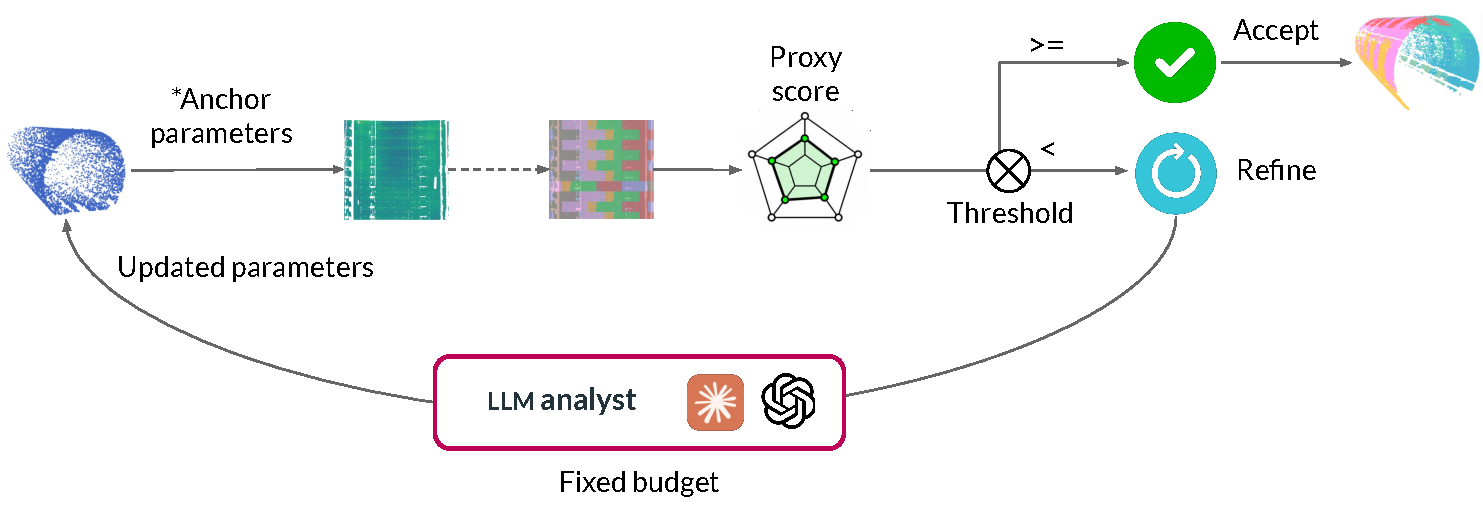
\includegraphics[width=0.9\textwidth]{figures/verification-1.pdf}
\caption{Proof-of-concept proxy verification. Each held-out subset is first
processed with the anchor parameters of its tunnel family and scored by the
learned proxy. Runs scoring at or above the acceptance threshold
($\tau = 0.7$) are accepted directly; otherwise an LLM agent, prompted with
the tunnel ontology, inspects the result and proposes updated parameters. The
loop repeats within a fixed refinement budget, after which the
highest-scoring configuration is retained. Accepted results are subsequently
evaluated against ground truth (mIoU).}
\label{fig:poc-workflow}
\end{figure*}

The final experiment tests whether the frozen proxy can drive a label-free
refinement loop (Fig.~\ref{fig:poc-workflow}). Each of five subsets is first
processed with its family anchor parameters and scored by the proxy. Runs
scoring at or above the acceptance threshold ($\tau = 0.7$) would be accepted
directly; below it, an LLM agent inspects the GT-free intrinsics and
artifacts, diagnoses deviations via the tunnel ontology, and proposes a
bounded multi-stage parameter overlay. Each round is re-scored by the proxy,
and after at most three rounds the highest-proxy configuration is retained.
The acceptance threshold is a deliberately conservative operating point on
the proxy score, distinct from the low-quality alarm threshold
($\tau = 0.495$) validated in Section~\ref{sec:main-results}: the former asks
``is this run good enough to ship without refinement?'', the latter ``is this
run bad enough to flag?''. Ground-truth mIoU is revealed only at final
evaluation and never enters the loop. Given the small sample ($n = 5$), we
report results per case and draw no statistical conclusions beyond
demonstrated feasibility.

\begin{table}[ht]
\caption{Proof-of-concept self-refinement: best-of-three reflection rounds
selected by proxy score, evaluated against ground truth only
afterwards.}\label{tab:poc-results}
\begin{tabular*}{\tblwidth}{@{} l c c c c @{}}
\toprule
Subset & Anchor mIoU & Selected mIoU & $\Delta$mIoU & Improved \\
\midrule
4-4 & 0.347 & 0.700 & $+$0.353 & yes \\
1-5 & 0.549 & 0.782 & $+$0.233 & yes \\
1-4 & 0.556 & 0.596 & $+$0.040 & yes \\
3-5 & 0.588 & 0.628 & $+$0.040 & yes \\
4-3 & 0.516 & 0.508 & $-$0.008 & no \\
\bottomrule
\end{tabular*}
\end{table}

\textbf{Selection by proxy improves four of five subsets.}
Table~\ref{tab:poc-results} summarises the campaign. Selecting the round with
the highest proxy score improves ground-truth mIoU on 4/5 subsets, with gains
from $+$0.040 to $+$0.353; the largest gain (subset 4-4, 0.347
$\rightarrow$ 0.700) doubles segmentation quality on a complex tunnel whose
anchor configuration under-detected ring boundaries. In each improved case
the round selected by proxy also improved ground-truth mIoU.

\begin{figure*}[t]
\centering
\begin{subfigure}{0.32\textwidth}
\centering
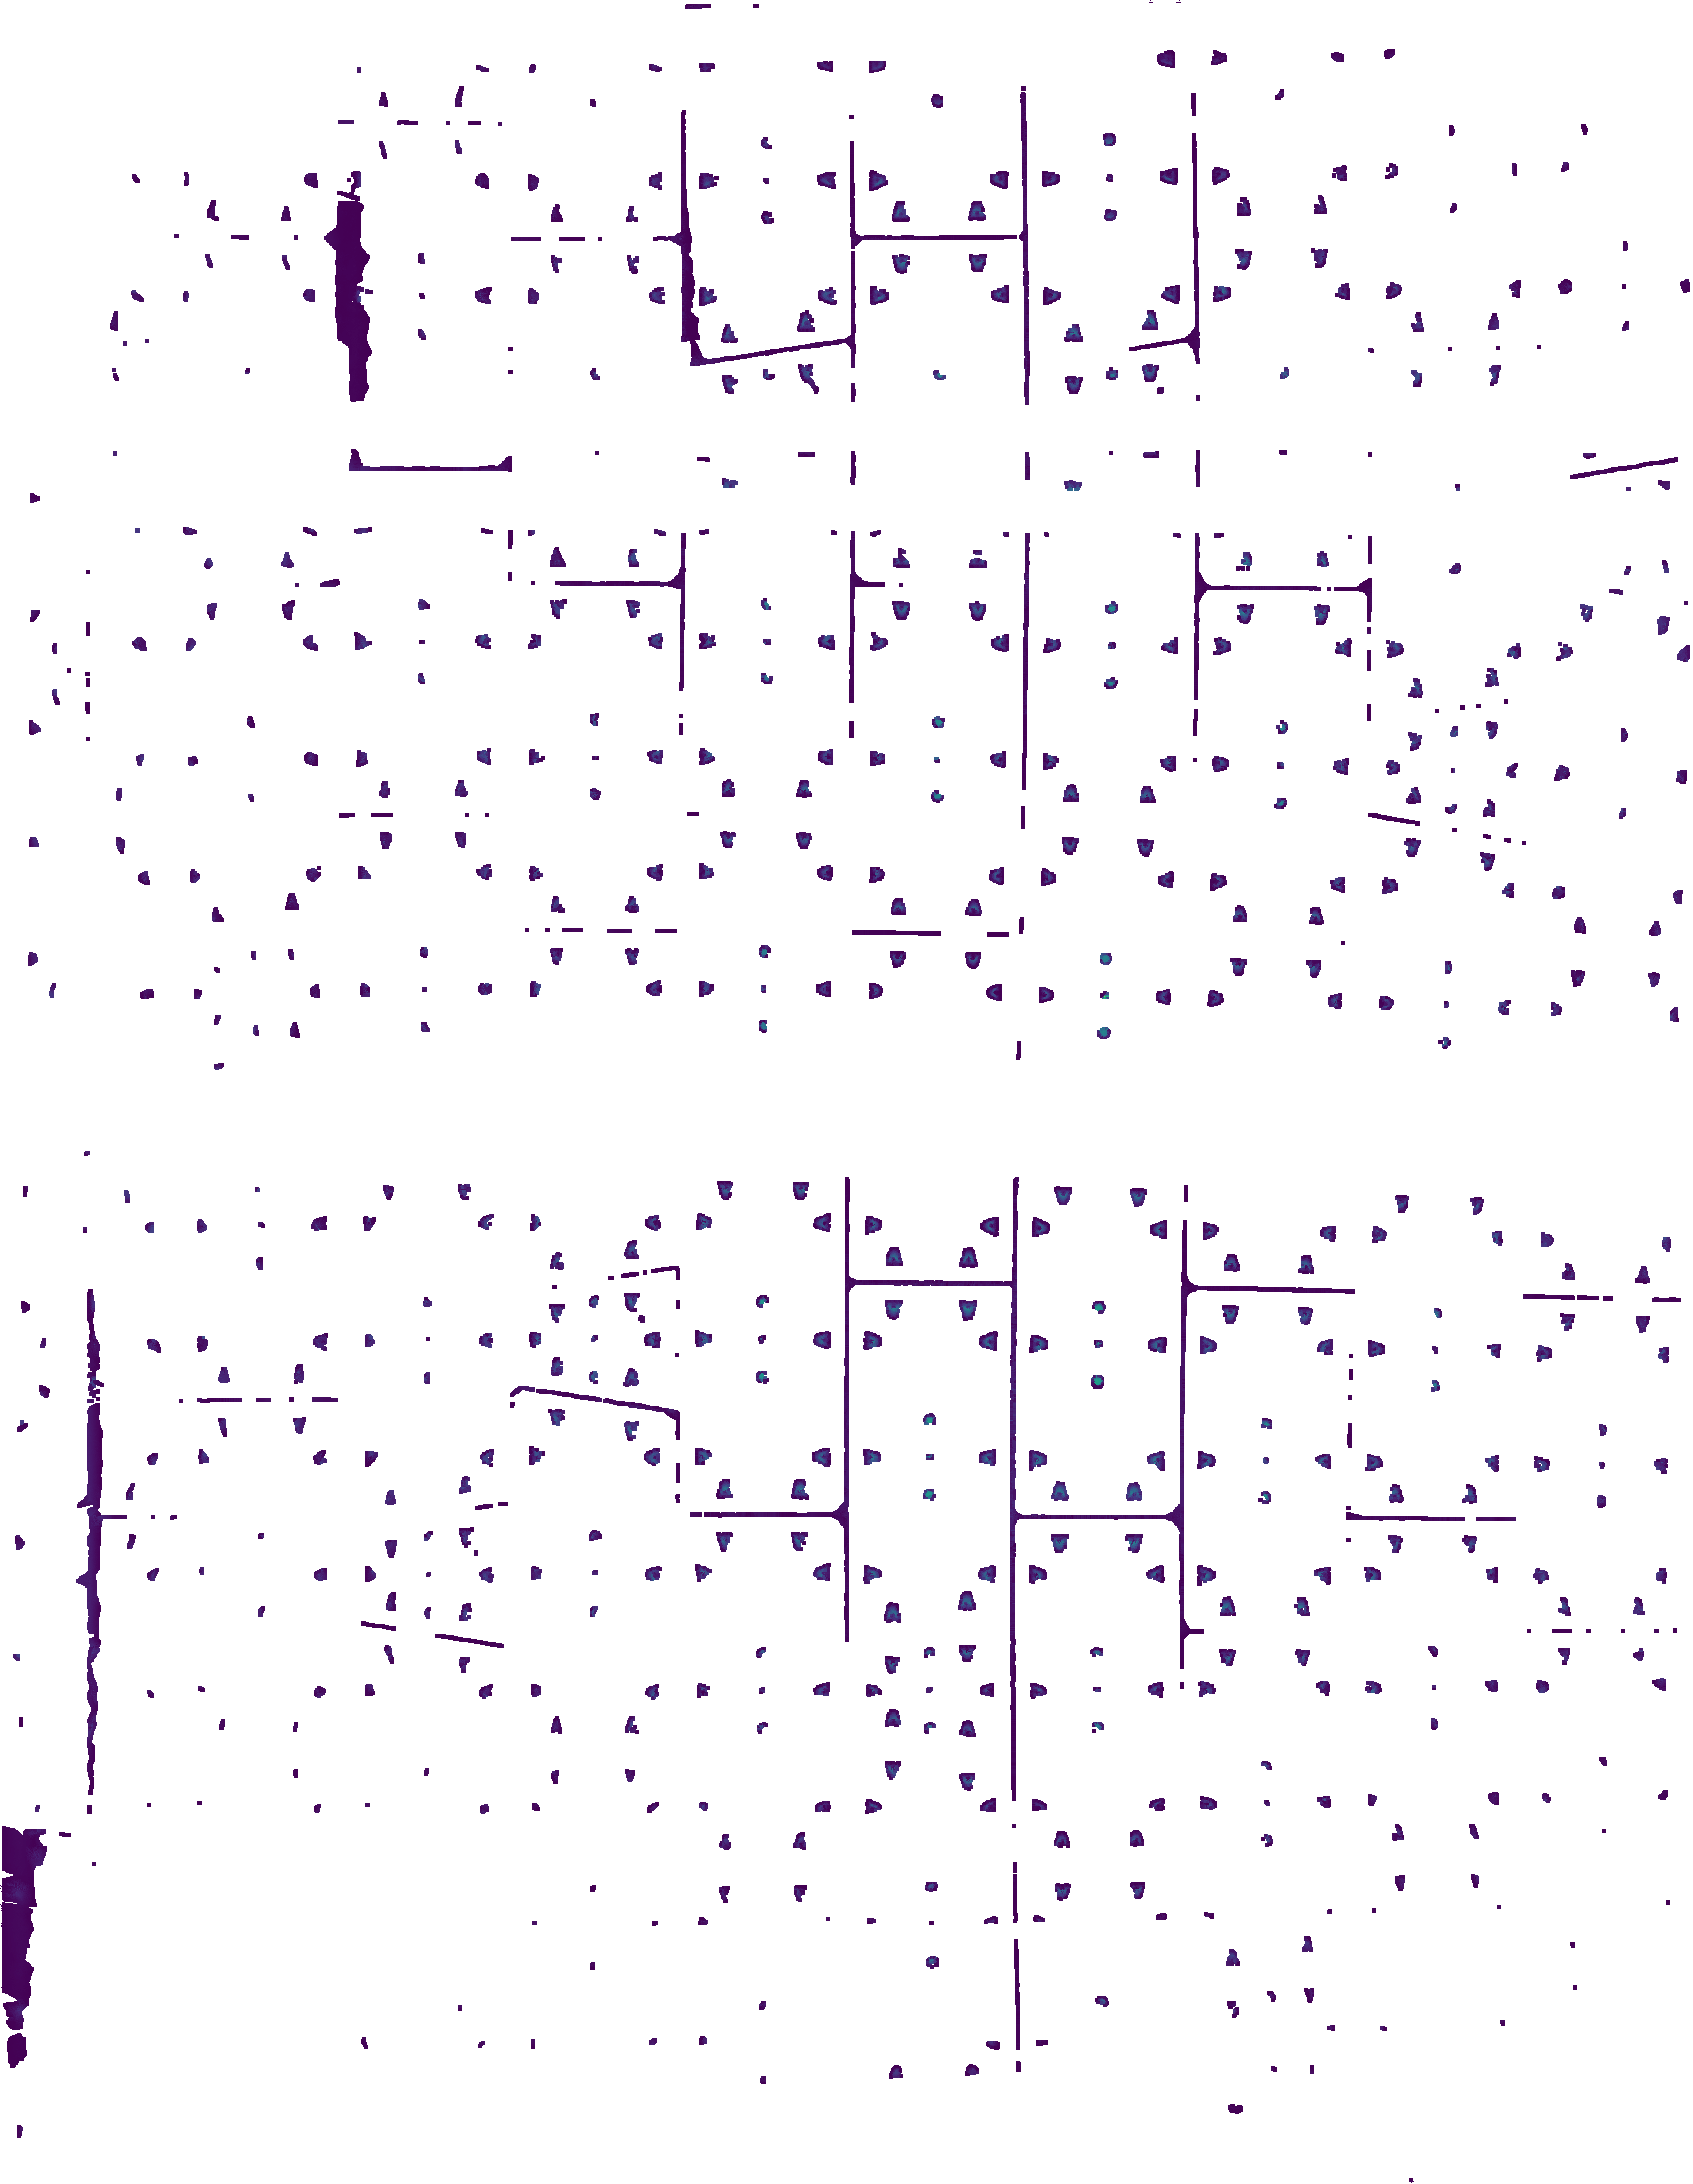
\includegraphics[width=\textwidth]{figures/5-1/low_depth_map.png}
\par\smallskip
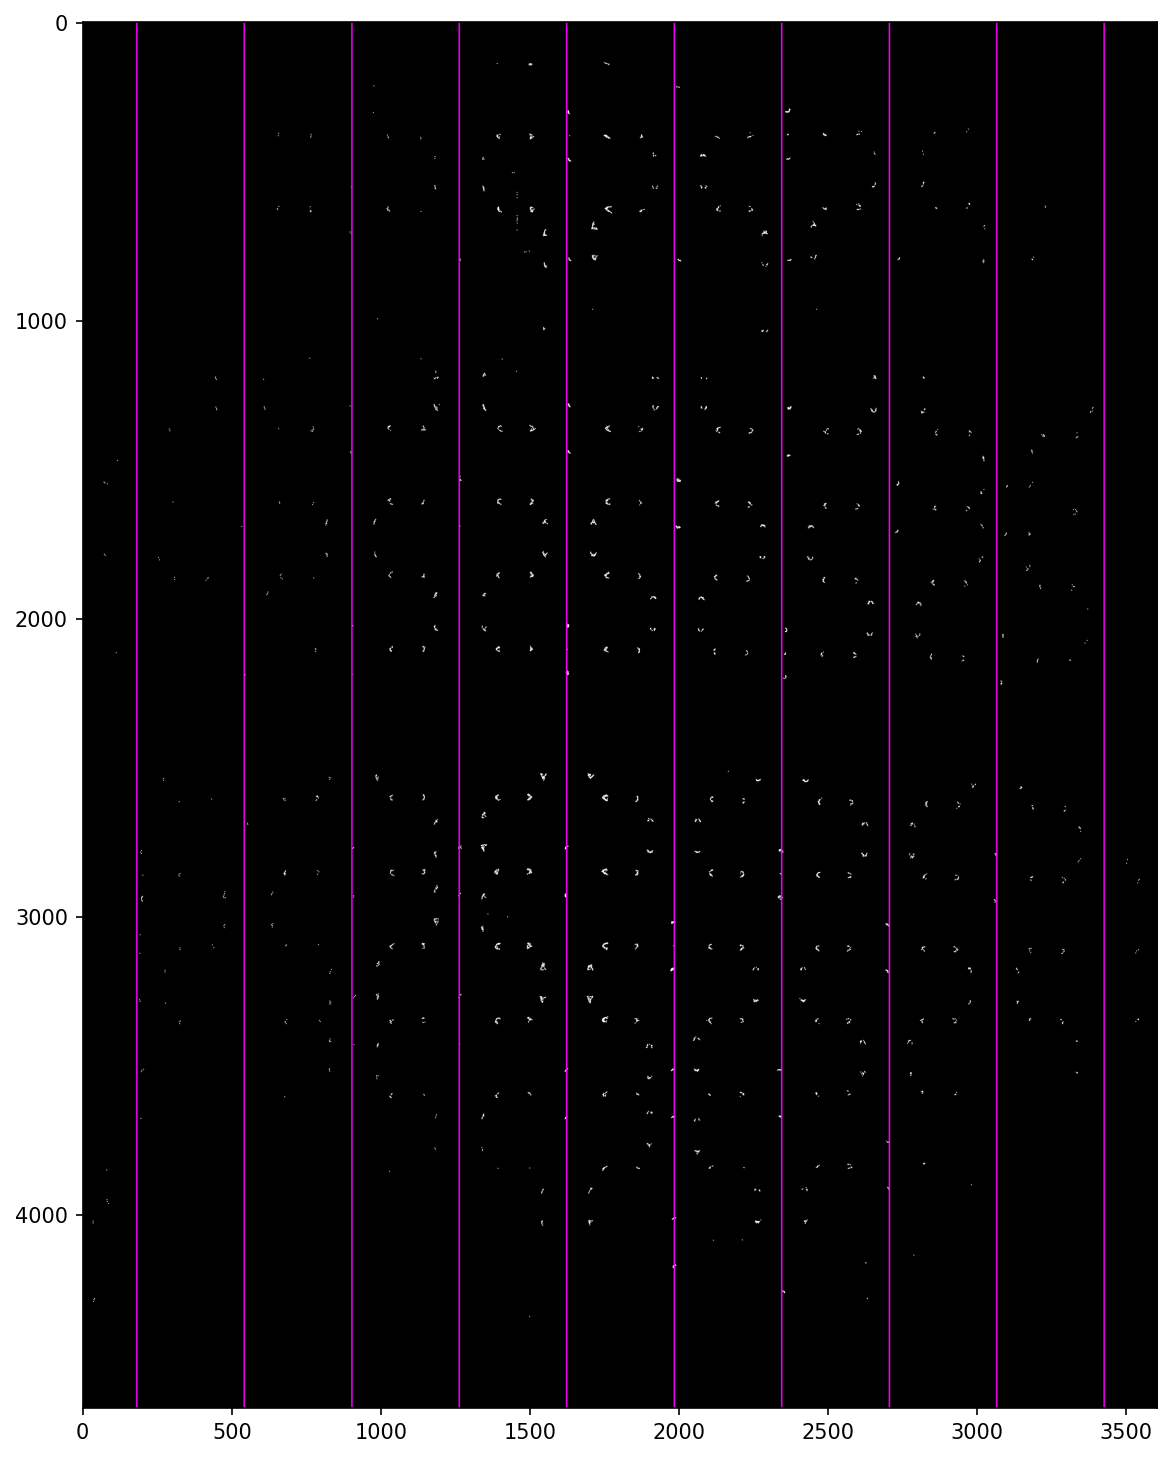
\includegraphics[width=\textwidth]{figures/5-1/low_detected_lines.png}
\par\smallskip (a) Low quality
\end{subfigure}
\hfill
\begin{subfigure}{0.32\textwidth}
\centering
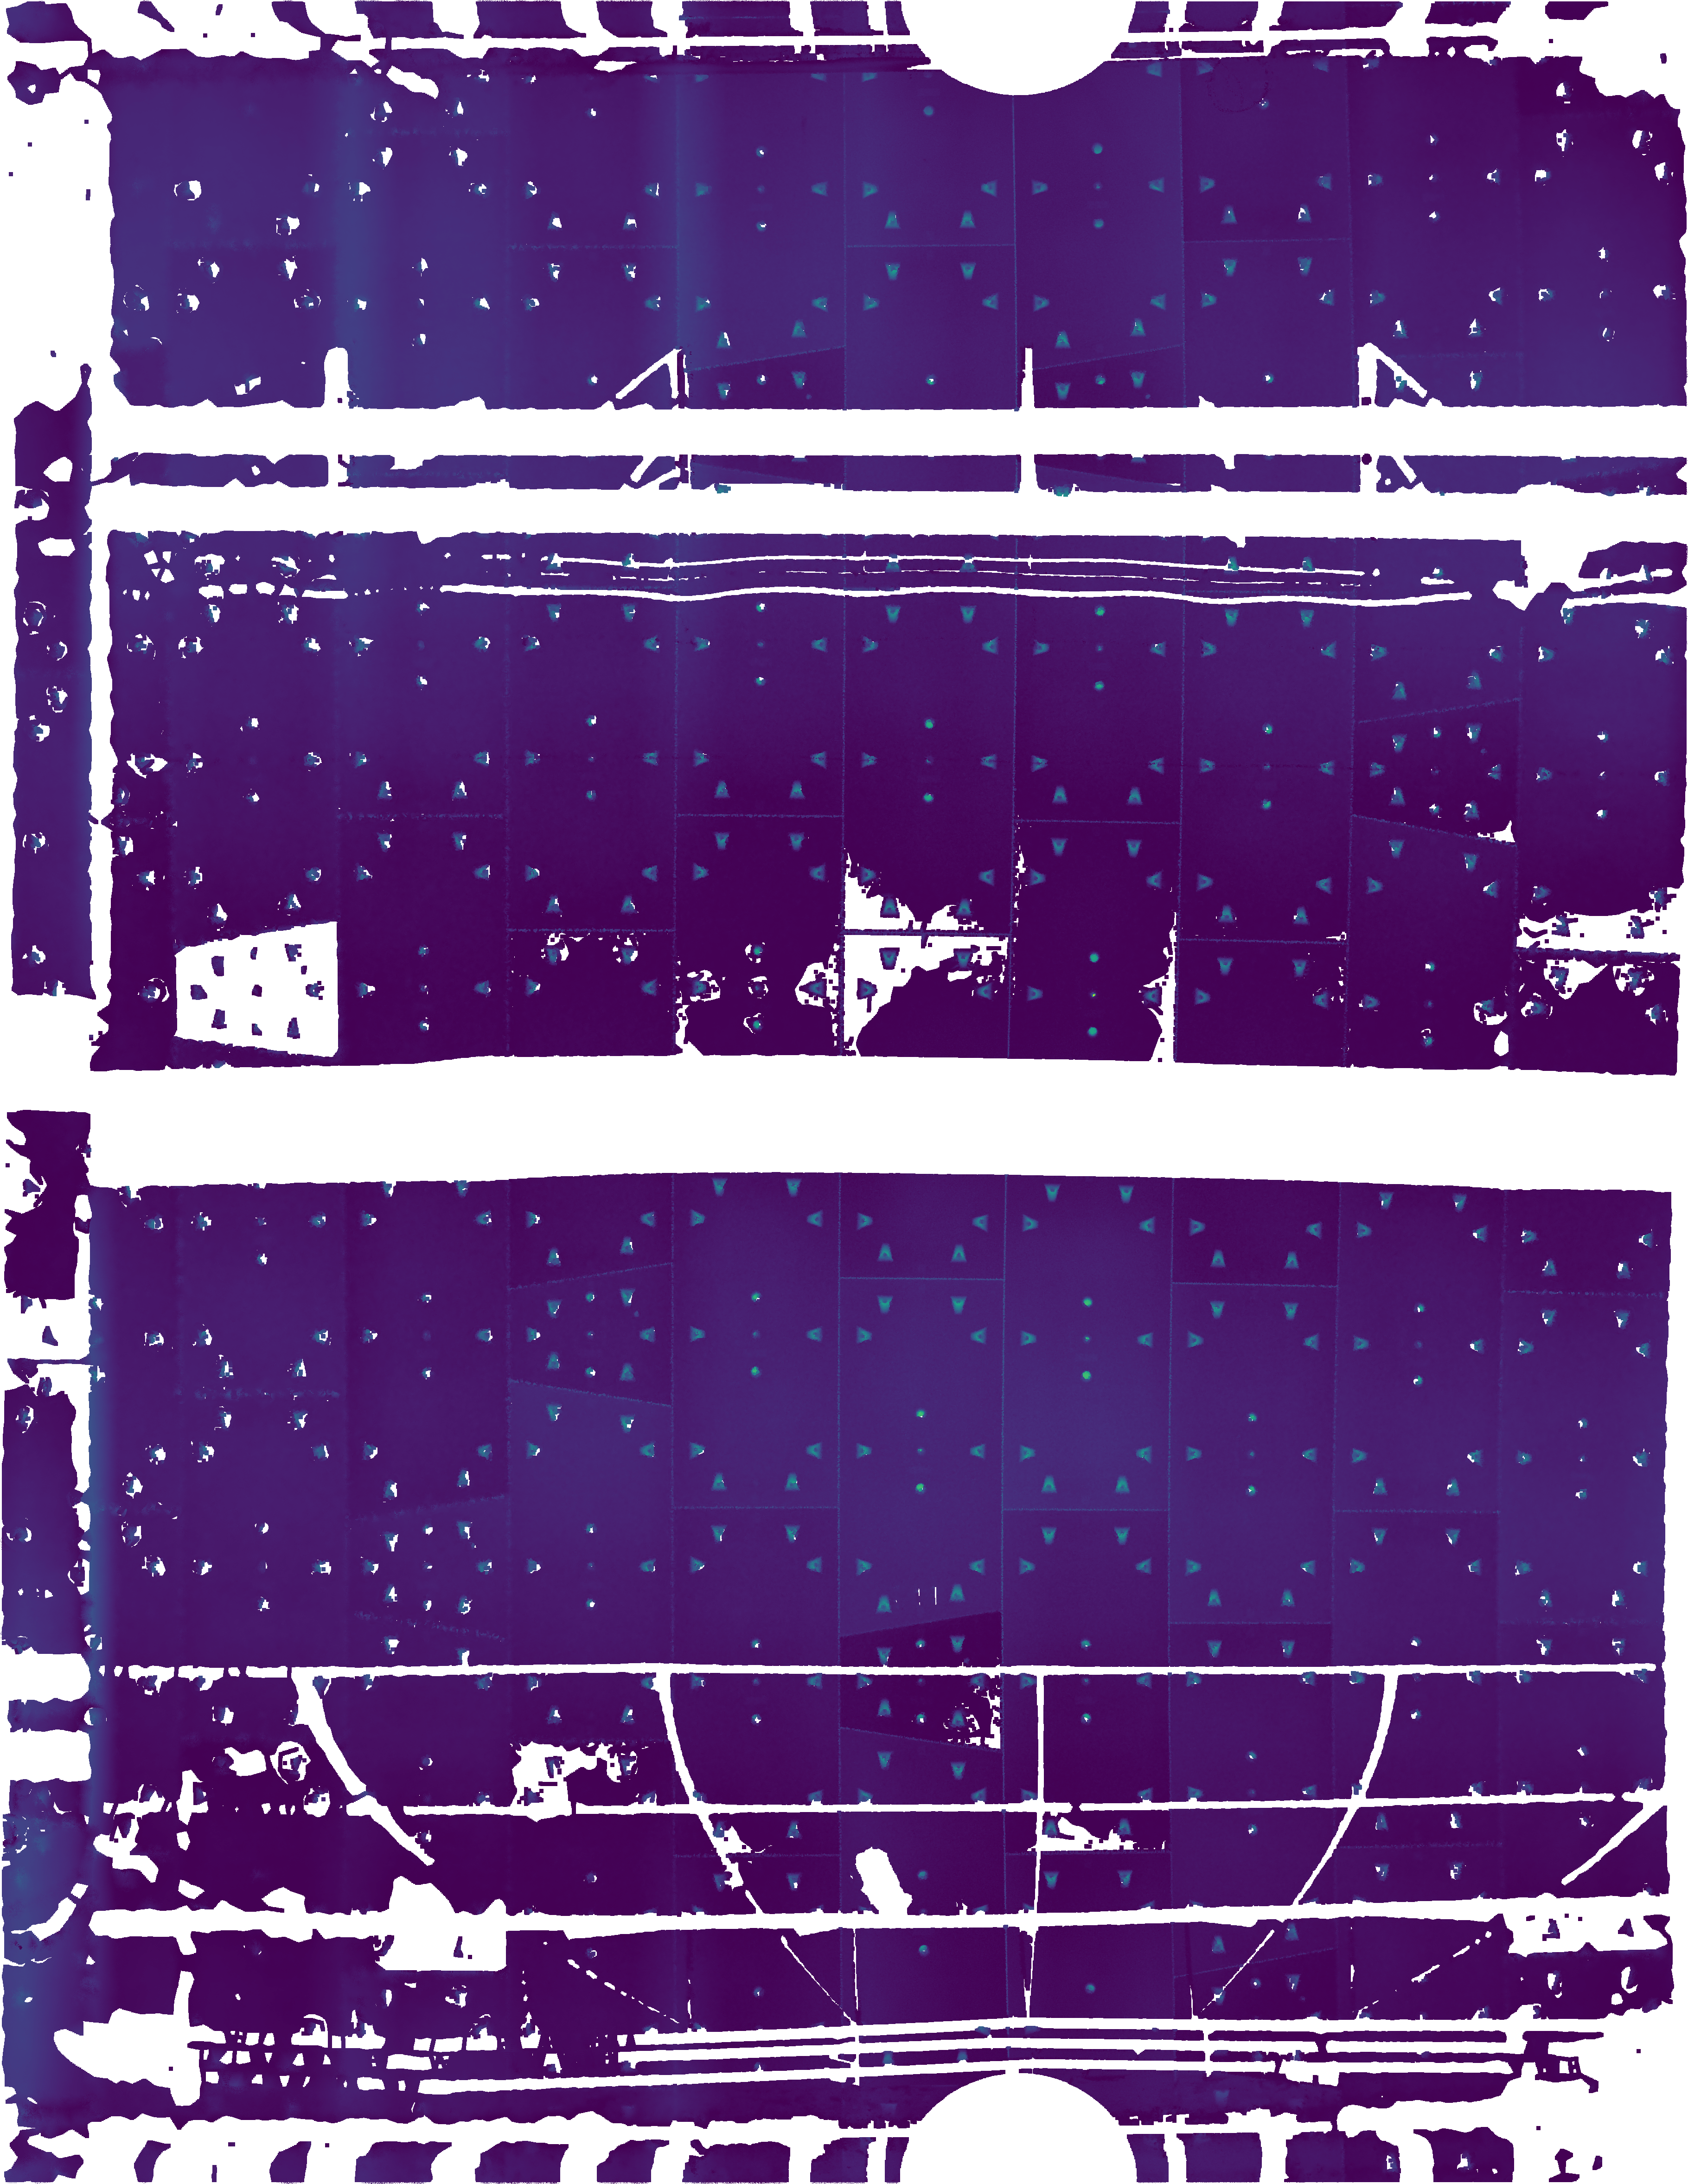
\includegraphics[width=\textwidth]{figures/5-1/mid_depth_map.png}
\par\smallskip
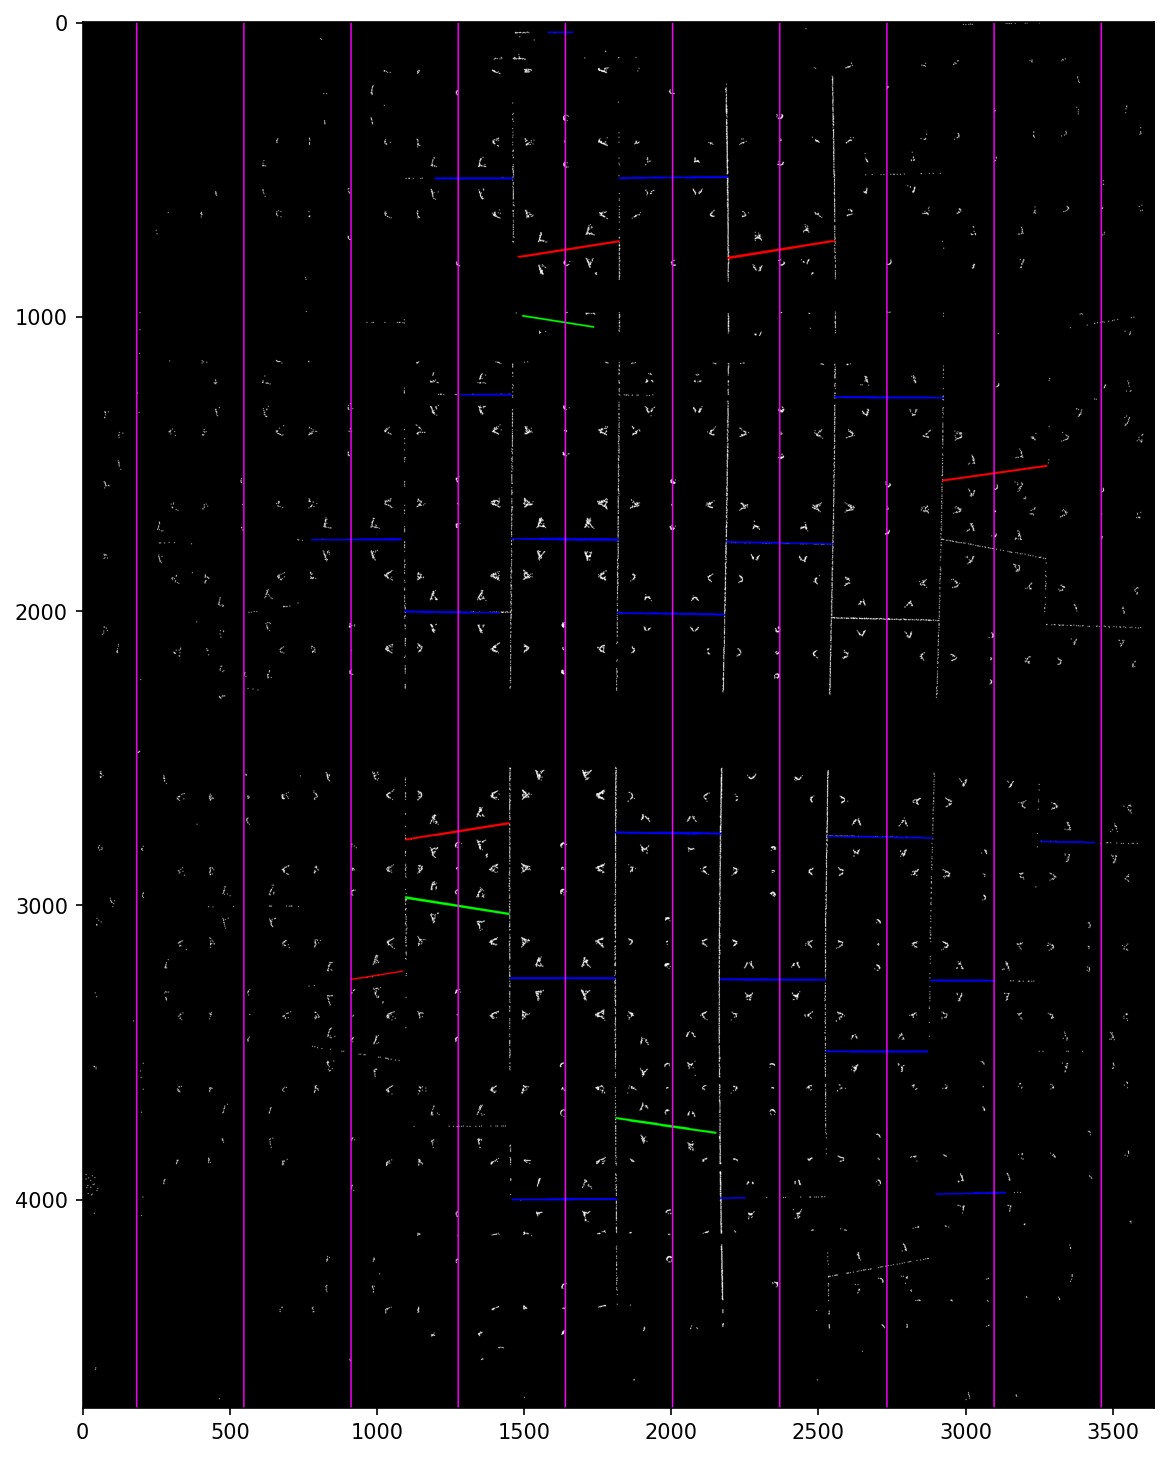
\includegraphics[width=\textwidth]{figures/5-1/mid_detected_lines.png}
\par\smallskip (b) Medium quality
\end{subfigure}
\hfill
\begin{subfigure}{0.32\textwidth}
\centering
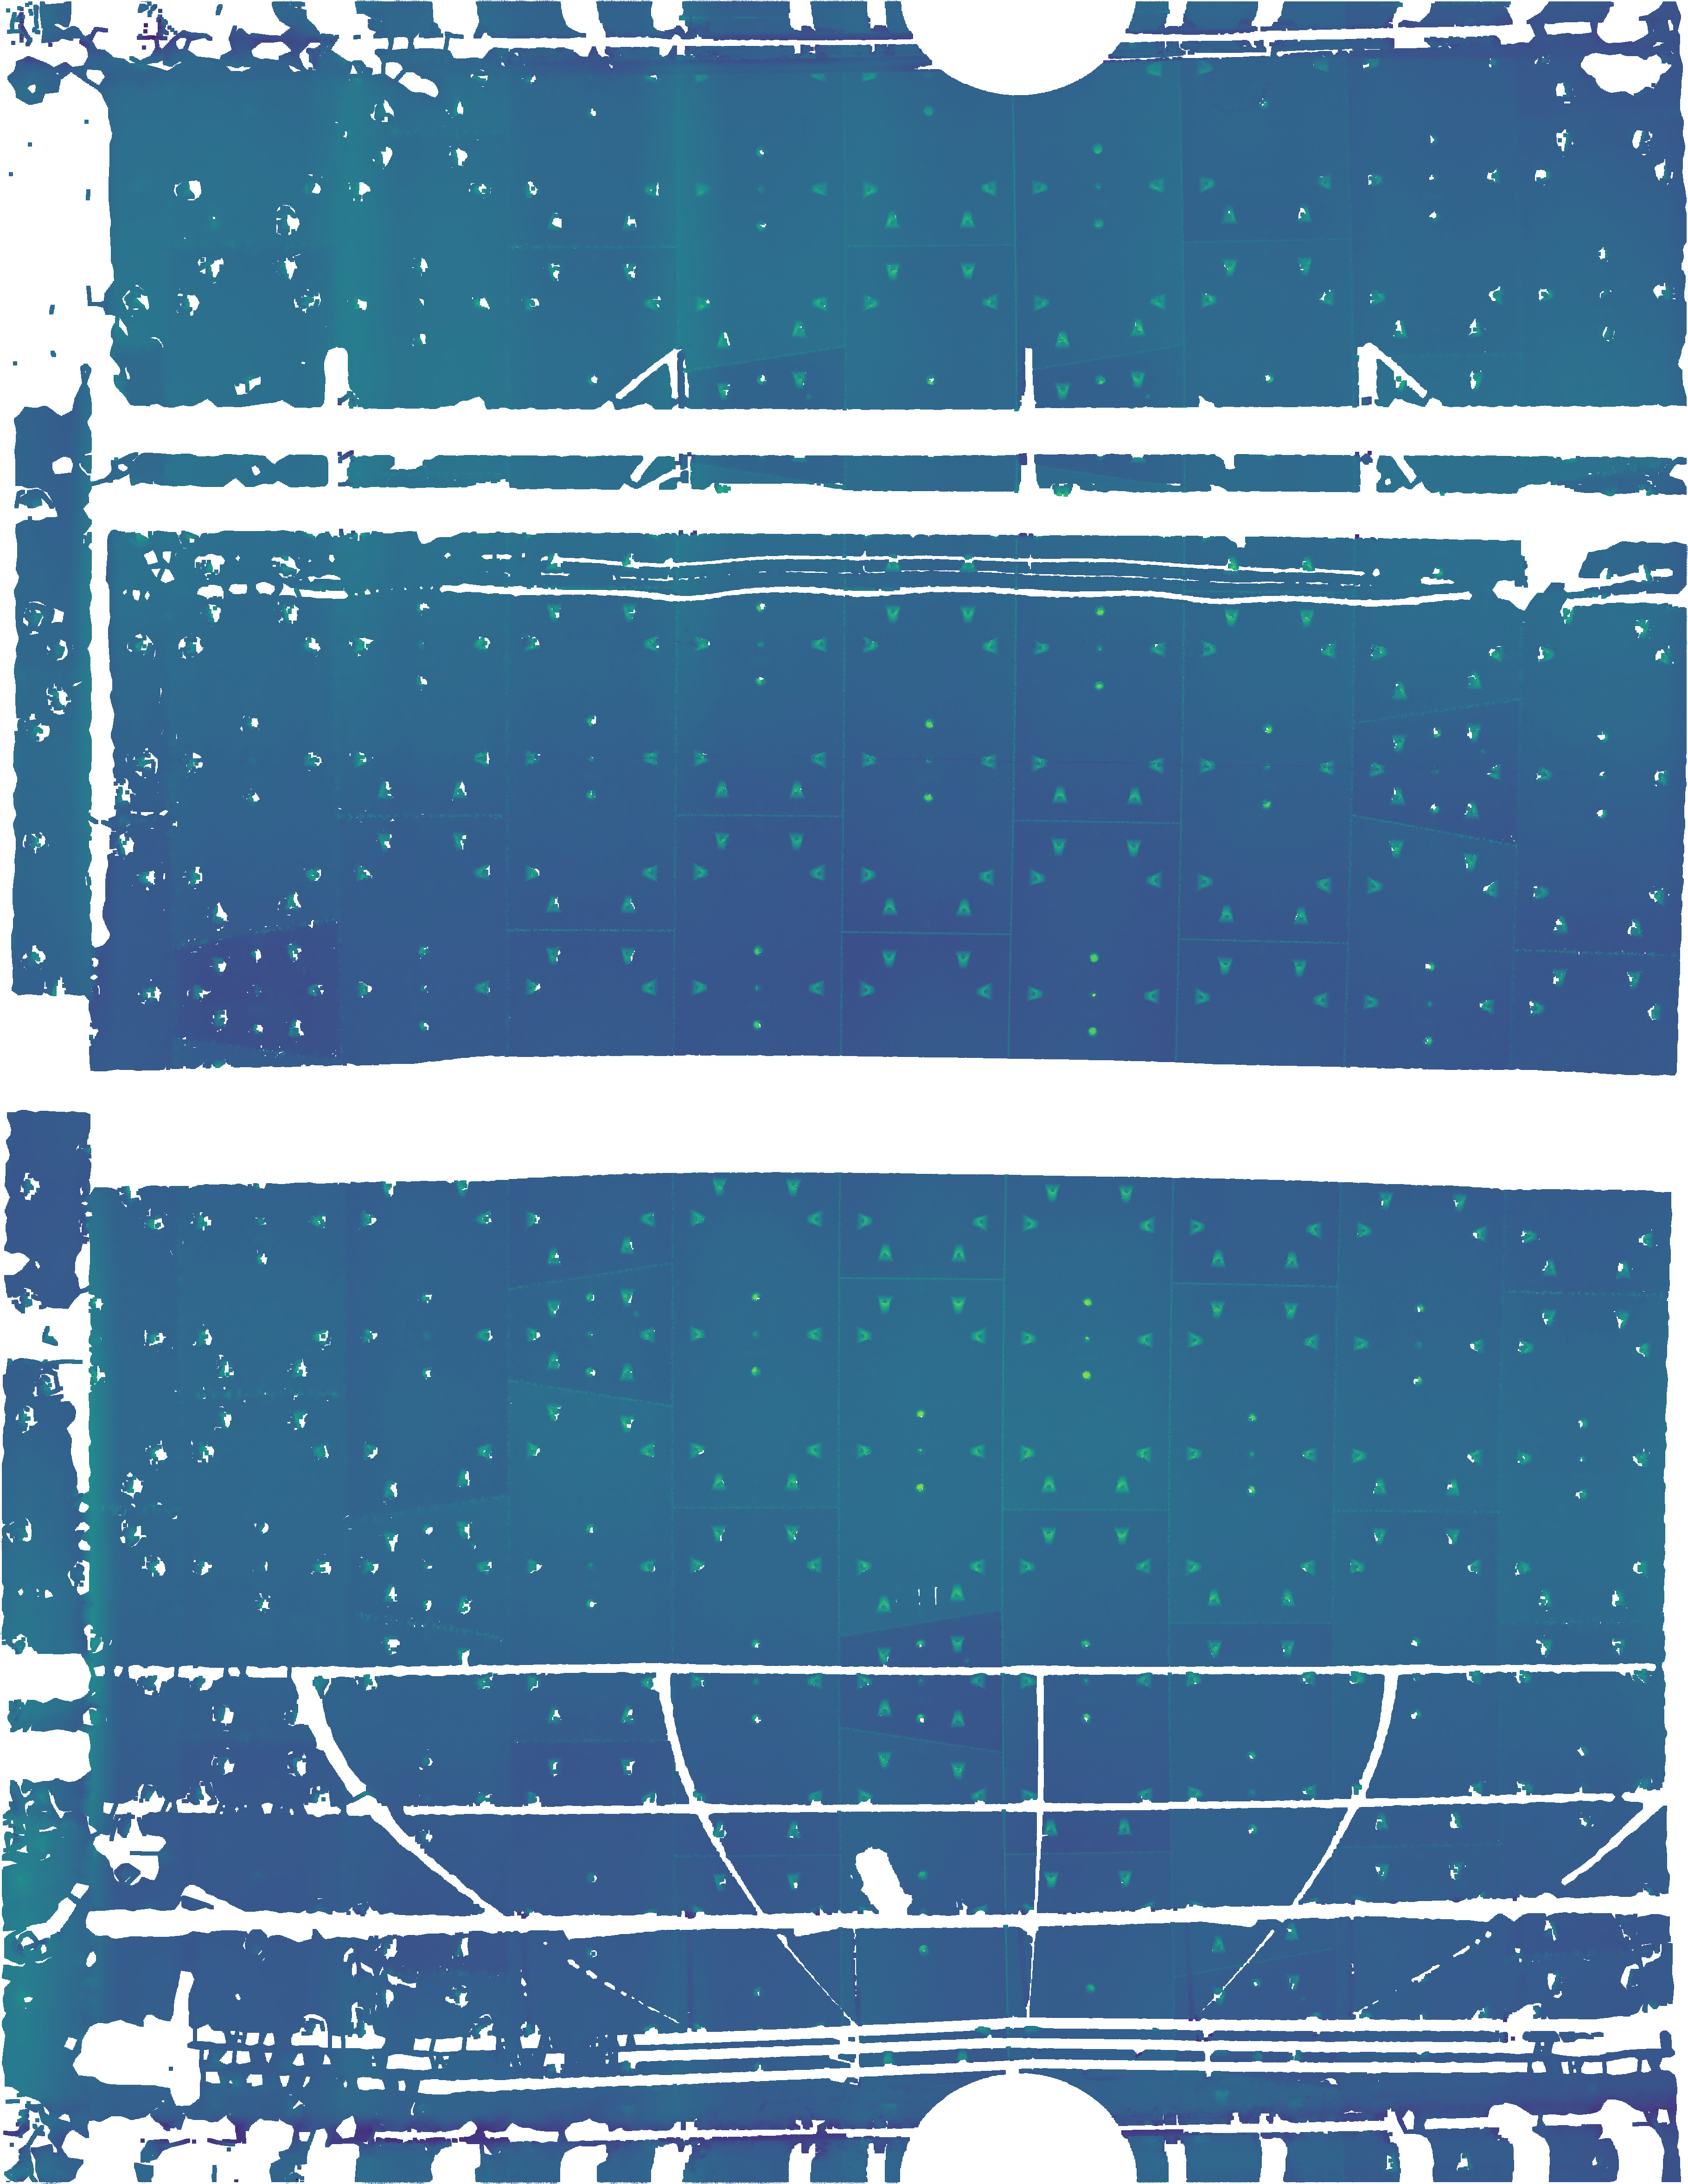
\includegraphics[width=\textwidth]{figures/5-1/best_depth_map.png}
\par\smallskip
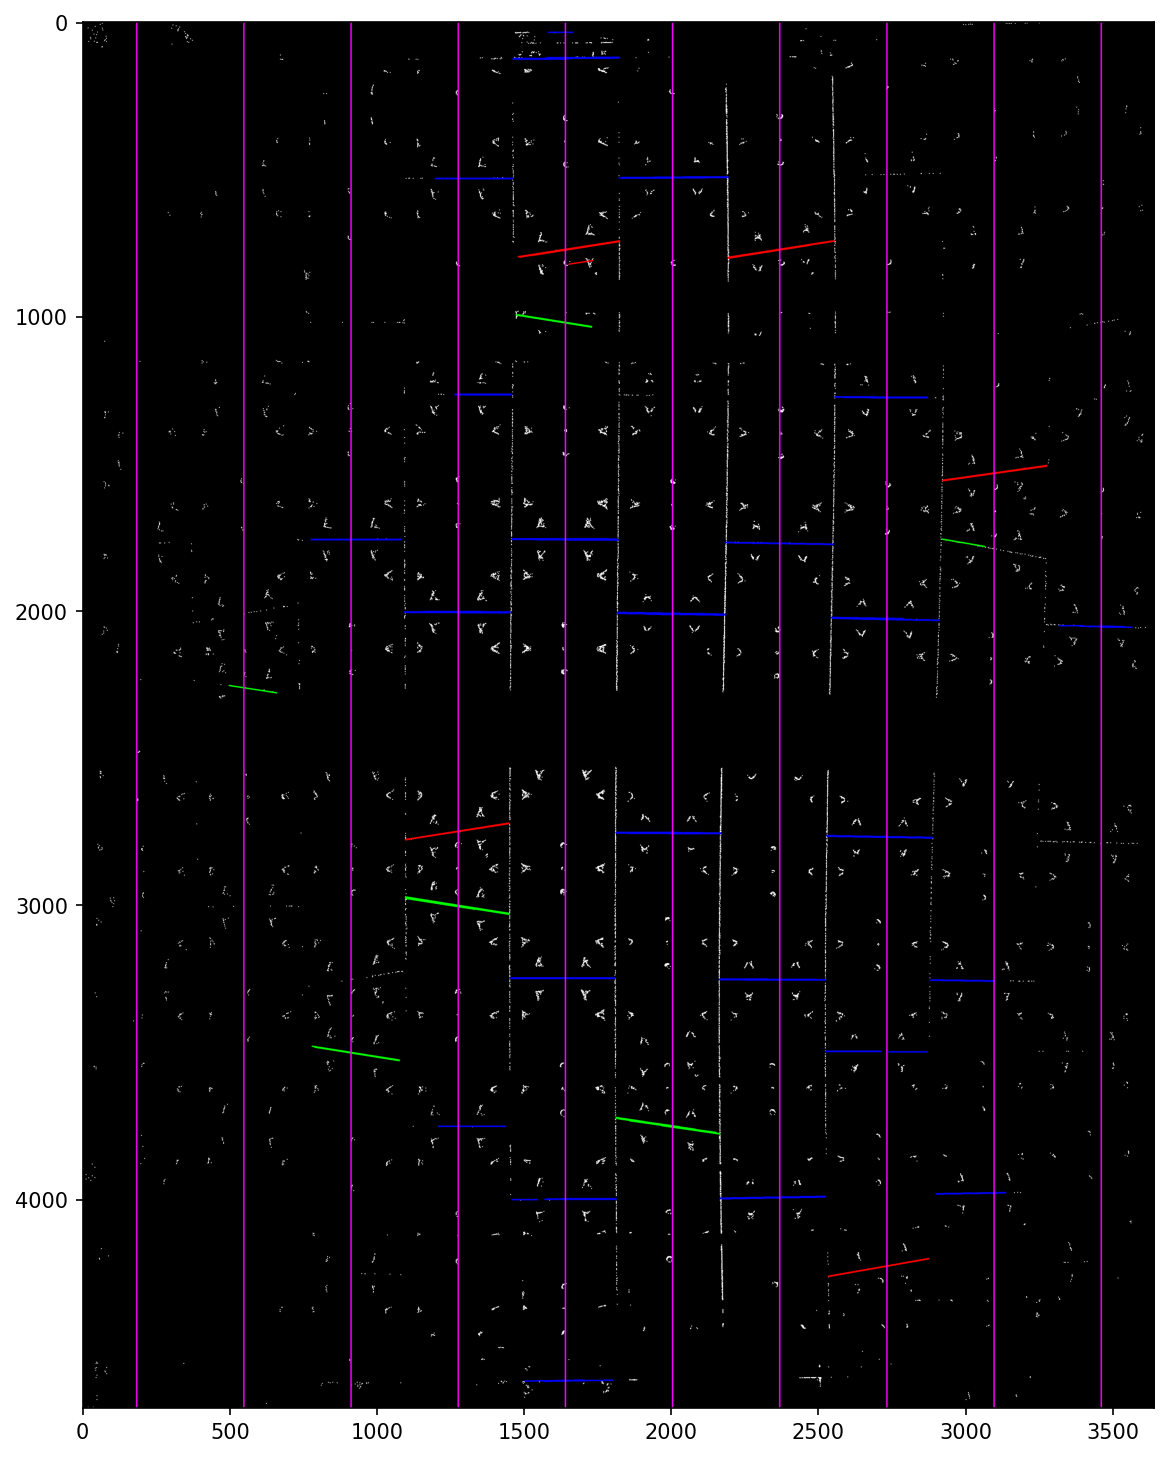
\includegraphics[width=\textwidth]{figures/5-1/best_detected_lines.png}
\par\smallskip (c) High quality
\end{subfigure}
\caption{What the proxy sees: unfolded depth maps (top) and detected joint
lines (bottom) for low-, medium-, and high-quality configurations of a
complex-family subset (5-1). Degraded configurations leave visible traces in
the artifacts --- incomplete depth coverage and irregular or missing joint
lines --- which the evidence and coherence features quantify without labels.}
\label{fig:poc-artifacts}
\end{figure*}

\textbf{Failure analysis: subset 4-3.} The one failure is diagnostic rather
than incidental. A ceiling probe over the stages 2--6 search space shows that
\emph{no} parameter overlay available to the reflection loop beats the anchor
on 4-3 (best manual configuration: $-$0.001; reflection best: $-$0.008): the
binding defect is the stage-1 centreline, whose recentring residual of
23.2\,cm distorts the unfolded geometry before any downstream parameter acts.
This quantity is invisible to the lean proxy --- substituting a healthy
residual into the 4-3 feature vector changes the prediction by exactly zero,
since the stage-1 candidates were pruned during feature ablation
(Section~\ref{sec:proxy-ablation-results}). When the loop is re-run with
stage~1 unlocked, changing the unfolding seed alone reduces the residual to
5.2\,cm and raises mIoU to 0.554 ($+$0.038 over the anchor), and all three
stage-1-aware rounds beat the anchor. The proxy thus delimits its own scope:
it reliably scores what the depth-map and segmentation artifacts reveal
(Fig.~\ref{fig:poc-artifacts}), and the 4-3 case identifies stage-1 geometry
auditing as the concrete extension required for a fully reflective agent.

\textbf{Scope of the claim.} This PoC is intended to demonstrate the proxy's
potential as a self-refinement signal for reflective LLM agents or
reinforcement learning, not to establish a general adaptation method: the
subsets were chosen to span families and failure modes, the refinement budget
was fixed at three rounds, and no hyperparameters were tuned on the outcome.
Within that scope, the loop shows that a frozen, five-feature linear proxy is
informative enough to select better configurations without any deployment
labels --- and, through its one failure, shows precisely where richer stage-1
evidence is needed.
